\documentclass[sigconf]{acmart}
\citestyle{acmauthoryear}
\AtBeginDocument{%
  \providecommand\BibTeX{{%
    \normalfont B\kern-0.5em{\scshape i\kern-0.25em b}\kern-0.8em\TeX}}}

\usepackage[utf8]{inputenc}



\begin{document}
\title{Position Based Fluid Simulation}

\author{Zhengyu Cai}
\affiliation{\institution{University of Toronto}}
\email{zhengyu.cai@mail.utoronto.ca}

\author{Yifeng He}
\affiliation{\institution{University of Toronto}}
\email{yifeng.he@mail.utoronto.ca}

\begin{abstract}
 This paper outlines a state-of-the-art approach for fluid simulation in both two and three dimensions. The algorithm that will be discussed in detail is entirely based on Miles Macklin and Matthias Muller’s paper “Position Based Fluids”. We will follow very closely with the pseudo code and method proposed in the paper and dive deep into the actual implementation and analysis to give readers a better understanding of the approach.
\end{abstract}

\maketitle

\section{Introduction}
Animating fluids like liquids, smoke and fire by physics-based animation plays an important role in visual effects in movies as well as games. For the past decades, scientists and researchers have come up with many techniques for simulating flows. Today we will be focusing on the position based (PBF) method as it is simpler, and more flexible over alternative approaches, most prominently the Eulerian method and traditional SPH. \\
In this project, we simulated liquid behaviour in a sealed container in both 2D and 3D scale. We interpret liquid as multiple gathering particles, and implemented the algorithm provided in "Position Based Fluids" [Macklin\&Muller13]. In this approach, we accumulate density and forces acting on each particles within a radius, use them to update the velocities and then positions of all the particles to finally show the simulation. The original algorithm is shown in 3D, but without applying XSPH viscosity it is applicable to 2D cases. Hence in our project and for both 2D and 3D version, we did not use the XSPH viscosity step. We also added a wall pusher mechanism to continuously move the particles around, simply to increase dramatic effect.

\section{Method}
In this section we will break down the simulation algorithm proposed in the original paper and discuss our approaches in detail. The first thing to cover is the equations of motion, which are relatively simple and straight-forward in our case. For each particle, we have: 
\begin{align*}
    v_i &= v_i + \delta tf_{ext}(x_i)
\end{align*}
where we only consider the gravity applied onto each particle, as $F_{ext} = g = (0.0, -9.8)$ or $(0.0, -9.8, 0.0)$ in 3D case (in our 3D implement the last axis represents depth). Then we predict the position for all the particles.

\subsection{Boundary}
After each position prediction, we use fix\_boundary() to make a check to all particles to make sure they stay within the designed area. The first approach: we could treat the boundary as many fixed particles. This means that when we calculate fluid particle densities ($\delta p$, $\lambda$) and take the boundaries particles into account. However, this would lead to heavy memory usage. As a result, in our implementation, we check if each particle is in contact with the boundaries and fix their positions. If they exceed the boundary, we fix them back to the boundary limit. Upon which we add a small randomized position change to that exceeding limit particle to avoid multiple particles stuck into one point and unexpected explosion behaviour due to extremely high density around one area.

\subsection{Neighbours}
In order to perform accumulation in later parts of the algorithm, we first need to find neighbours of each particles. A naive approach is to loop through all pairs of particles and retrieve minimum distance particles as neighbours to each particle, which takes a not very efficient complexity of $\mathcal{O}(n^2)$. We implemented a hashing method from open-source[2] as explained below. \\
For the simulation world we split them into square cells of size 2x2 to form a grid. We loop through all particle to make a hash-table that records which cell that particle belongs to in the grid. For each particle, we find which cell it belongs to, and find neighbour particles from its surrounding cells. As a result we check $3*3=9$ cells of particles in 2D while $3*3*3=27$ in 3D. To make the algorithm consistent, we only consider first 100 particles found in one cell in the world, and first 50 valid particles taken to be a particle's neighbour. This way our implemented algorithm takes $\mathcal{O}(9*100n) = \mathcal{O}(n)$ in 2D and similar for 3D.

\subsection{Enforcing Incompressibility}
While enforcing incompressibility is costly in the SPH approach, this constraint can fit easily in PBF. Recall that in an incompressible system, we should keep each particle’s density to be the same as its rest density. From SPH, the density estimator is given by: 
\begin{align*}
    \rho_i &=\sum_j m_jW(p_i-p_j, h)\\
    W_{poly6}(r, h) &= \frac{315}{64\pi h^9}\begin{cases}
            (h^2-r^2)^3 & 0\leq r \leq h\\
            0 & \mbox{otherwise} 
        \end{cases}
\end{align*}
where $W= W_{poly6}(r, h)$ is poly6 kernel from [Muller et al. 03].
Following detailed calculations from the original paper, the updated position $\Delta p_i$ including corrections from neighbor particles density constraint $\lambda_j$ is:
\begin{align*}
    \lambda_i &= -\frac{C_i(p_1,...,p_n)}{\sum_k |\nabla p_kC_i|^2 + \epsilon}\\
    \delta p_i &= \frac{1}{\rho_0}\sum_j(\lambda_i + \lambda_j)\nabla W(p_i - p_j, h)
\end{align*}
where $\nabla W$ is the gradient of the spiky kernel from [Muller et al. 03] as 
\begin{align*}
    W_{spiky}(r, h) = \frac{15}{\pi h^6}\begin{cases}
            (h-r)^3 & 0\leq r \leq h\\
            0 & \mbox{otherwise} 
        \end{cases}
\end{align*}
\subsubsection{$W_{poly6}$ V.S. $W_{spiky}$:}
Note that $r$ appears squared in this $W_{poly6}$, meaning that there is no need to take square roots in distance calculation. However, this kernel produces funky results under high pressure due its gradient being zero at the center. Hence the authors use Debrun’s spiky kernel $W_{spiky}$ for gradient calculation.

\subsection{Tensile Instability}
In traditional SPH approach, when particles have too few neighbors, their densities fail to satisfy incompressibility, lead to particles clumping together. To resolve this, we add an artificial pressure term $s_{corr}$ which follows the approach of [Monaghan 2000]:
\begin{align*}
    s_{corr} = -k(\frac{W(p_i-p_j, h)}{W(\delta q, h)})^n
\end{align*}
where $W$ is the poly6 kernel [Muller et al. 03] and $\delta q$ is a point in some fixed distance inside the smoothing kernel radius. Based on the original paper, we take $|\delta q| = 0.2 h$ and $n=4$. We modified $k=0.001$ to make best performance as the numerical scale of our world is rather small. Finally by taking this artificial pressure term into position update function we use Eq(14) in [Macklin\&Muller13]:
\begin{align*}
    \delta q_i = \frac{1}{\rho_0}\sum_j(\lambda_i + \lambda_j + s_{corr})\nabla W(p_i-p_j, h)\\
\end{align*}
We repeat the previous two steps 5 times to get a better positioning of particles, without costing too much time and memory.

\subsection{Update}
Finally we update the position based on previous calculated $\delta q$ to each particle, and update their "new" velocity to be $\frac{1}{\delta t}(x_i^* - x_i)$ as if we determine the particle's velocity is based on the two "time-frame" positions.

\subsection{Pusher}
We added a moving boundary in 2D, and a moving wall in 3D that moves back and forth to create some dramatic effect on the fluid. The pusher is set to be a new boundary that will be checked in the boundary detection mechanism mentioned in section 2.1.

\section{Results}
We used Taichi embedded in python on GPU with multiple threading to increase the performance. For our 2D version, we simulated 1000 particles within a rectangular container and used Taichi Gui to render the result. For our 3D version, we simulated 2500 particles and used taichi to export each 3D frame (which contains all 3d-positions of all particles in the time frame) into PLY files, then use Houdini to rebuild the whole 3d animation. We can only view 2D scene in real time but not 3D as it needs to be built up. Below shown some result snapshots.\\ 
\begin{center}
    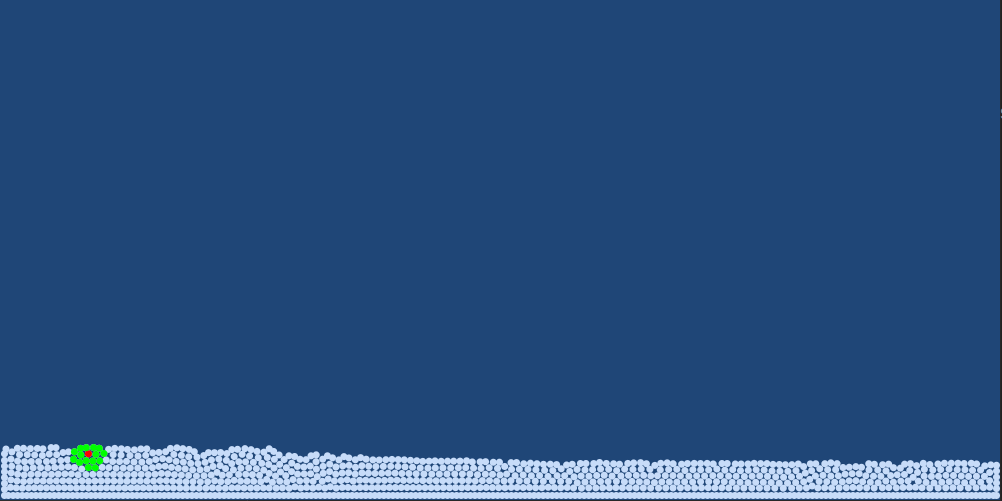
\includegraphics[width=4cm]{1.png} 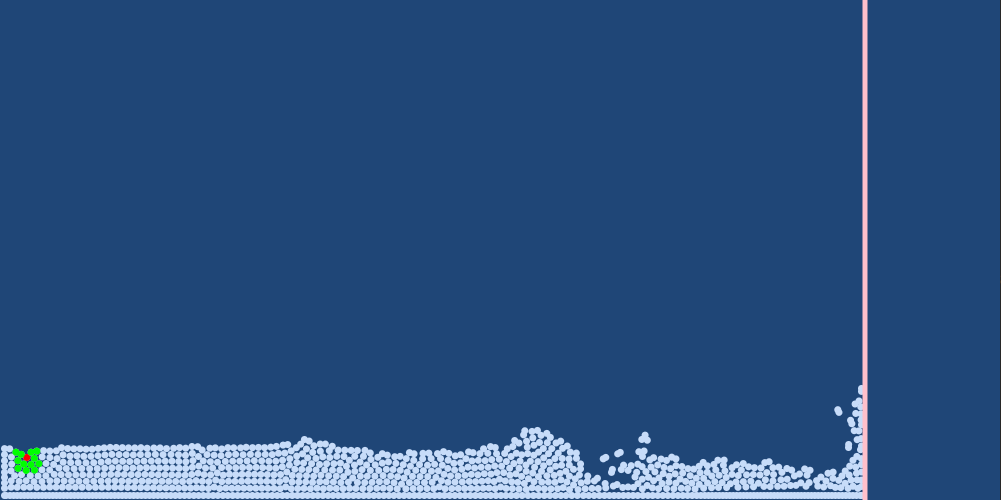
\includegraphics[width=4cm]{2.png} \\
    stable 2d fluid vs pushed 2d fluid
\end{center}
\begin{center}
    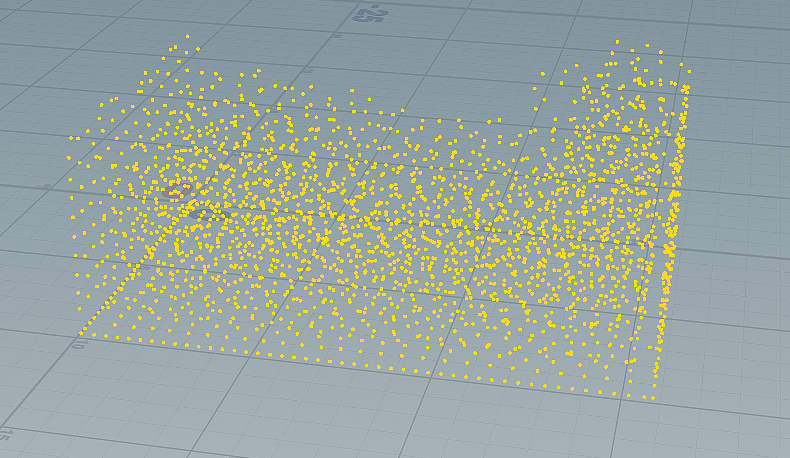
\includegraphics[width=5cm]{3.png}\\
    3d snapshot
\end{center}
A full demo video can be found in the video.

\section{Conclusion}
Overall both 2d and 3d simulation looks convincing, as algorithm in [Macklin\&Muller13] turns out to be simple but efficient. While enforcing incompressibility is computationally expensive for alternative approaches, e.g. traditional SPH approach. We have proven that this constraint can fit very well in the PBF model.

\section{References}
(1) MACKLIN, M., MULLER, M. 2013. Position Based Fluids. ACM Transactions on Graphics, vol.32, no.4, pp1-12, 2013\\\\
(2) InteractiveComputerGraphics. (n.d.). InteractiveComputerGraphics/Positionbaseddynamics: Positionbaseddynamics is a library for the physically-based simulation of rigid bodies, deformable solids and fluids. from https://github.com/InteractiveComputerGraphics/P\\ositionBasedDynamics\\\\
(3) MONAGHAN, J. J. 2000. Sph without a tensile instability. J.Comput. Phys. 159, 2 (Apr.), 290–311.\\\\
(4) MULLER, M., HEIDELBERGER, B., HENNIX, M., AND RATCLIFF, J. 2007. Position based dynamics. J. Vis. Comun. Image Represent. 18, 2 (Apr.), 109–118.\\\\
(5) MULLER, M., CHARYPAR, D., AND GROSS, M. 2003. Particlebased fluid simulation for interactive applications. In Proceedings of the 2003 ACM SIGGRAPH/Eurographics symposium on Computer animation, Eurographics Association, Aire-la-Ville, Switzerland, Switzerland, SCA ’03, 154–159.
\end{document}
\endinput

